% Copyright 2004 by Till Tantau <tantau@users.sourceforge.net>.
%
% In principle, this file can be redistributed and/or modified under
% the terms of the GNU Public License, version 2.
%
% However, this file is supposed to be a template to be modified
% for your own needs. For this reason, if you use this file as a
% template and not specifically distribute it as part of a another
% package/program, I grant the extra permission to freely copy and
% modify this file as you see fit and even to delete this copyright
% notice. 

\documentclass{beamer}

% There are many different themes available for Beamer. A comprehensive
% list with examples is given here:
% http://deic.uab.es/~iblanes/beamer_gallery/index_by_theme.html
% You can uncomment the themes below if you would like to use a different
% one:
%\usetheme{AnnArbor}
%\usetheme{Antibes}
%\usetheme{Bergen}
%\usetheme{Berkeley}
%\usetheme[hideothersubsections]{Berkeley}
%\usetheme{Berlin}
%\usetheme{Boadilla}
%\usetheme{boxes}
%\usetheme{CambridgeUS}
%\usetheme{Copenhagen}
%\usetheme{Darmstadt}
%\usetheme{default}
%\usetheme{Frankfurt}
%\usetheme{Goettingen}
\usetheme{Hannover}
%\usetheme{Ilmenau}
%\usetheme{JuanLesPins}
%\usetheme{Luebeck}
%\usetheme{Madrid}
%\usetheme{Malmoe}
%\usetheme{Marburg}
%\usetheme{Montpellier}
%\usetheme{PaloAlto}
%\usetheme{Pittsburgh}
%\usetheme{Rochester}
%\usetheme{Singapore}
%\usetheme{Szeged}
%\usetheme{Warsaw}

\title{Bayesian Deep Learning with 10 \% of the weights}
\subtitle{Practical approach to Bayesian deep learning}
\author{Rob Romijnders}

\institute[Universities of Somewhere and Elsewhere] % (optional, but mostly needed)
{
  \mdlink{robromijnders.github.io}{http://robromijnders.github.io/}}
% - Use the \inst command only if there are several affiliations.
% - Keep it simple, no one is interested in your street address.

\date{PyData Amsterdam, 2018}
% - Either use conference name or its abbreviation.
% - Not really informative to the audience, more for people (including
%   yourself) who are reading the slides online

\subject{Bayesian Deep Learning}
% This is only inserted into the PDF information catalog. Can be left
% out. 

% If you have a file called "university-logo-filename.xxx", where xxx
% is a graphic format that can be processed by latex or pdflatex,
% resp., then you can add a logo as follows:

% \pgfdeclareimage[height=0.5cm]{university-logo}{university-logo-filename}
% \logo{\pgfuseimage{university-logo}}

% Delete this, if you do not want the table of contents to pop up at
% the beginning of each subsection:
\AtBeginSubsection[]
{
  \begin{frame}<beamer>{Outline}
    \tableofcontents[currentsection,currentsubsection]
  \end{frame}
}
\usepackage{hyperref}
\newcommand{\fitfigure}[1]{\centering\includegraphics[width=\linewidth,height=0.7\textheight,keepaspectratio]{#1}}
\newcommand{\mdlink}[2]{\href{#2}{\underline{#1}}}
\newcommand{\undermath}[2]{\underbrace{#1}_\text{#2}}

\usepackage{listings}
\lstset{breaklines}
\usepackage{animate}
\usepackage{url}
\usepackage{mathtools}% Loads amsmath
\usepackage{lipsum}
\usepackage{caption}
\captionsetup{font=footnotesize}





% Let's get started
\begin{document}

\begin{frame}
	\titlepage
\end{frame}

\begin{frame}{Outline}
	\tableofcontents
	% You might wish to add the option [pausesections]
\end{frame}

% Section and subsections will appear in the presentation overview
% and table of contents.
\section{Introduction}

\subsection{Motivation}

\begin{frame}{Problems with neural networks}
	\centerline{Neural networks have two problems:}
	\centerline{  }
	\begin{enumerate}
		\item Neural networks give no \textbf{uncertainty} in predictions \\ 
		      \quad \quad \small{ $\rightarrow$ easily fooled by \textbf{adversarial examples}}
		\item Neural networks have \textbf{millions of parameters}
	\end{enumerate}
\end{frame}

\begin{frame}{Motivation}
	\begin{figure}
		\fitfigure{im/xray.png}
		\caption{Uncertainty is important when making diagnoses}
	\end{figure}
\end{frame}

\begin{frame}{Motivation}
	\begin{figure}
		\fitfigure{im/autonomous_driving.jpg}
		\caption{Uncertainty is important when making a critical decision}
	\end{figure}
\end{frame}

\begin{frame}{Motivation}
	\begin{figure}
		\fitfigure{im/bitcoin.png}
		\caption{Uncertainty is important when prediction bitcoin}
	\end{figure}
\end{frame}

\begin{frame}{Adversarial attack}
	\begin{figure}
		\fitfigure{im/adversarial_attack.jpeg}
		\caption{Uncertainty is necessary to find adversarial examples}
	\end{figure}
\end{frame}

\begin{frame}{Embedded applications}
	\begin{figure}
		\fitfigure{im/raspberry_pi.jpg}
		\caption{Pruning reduces the memory and computation usage  (Pruning = dropping parameters)}
	\end{figure}
\end{frame}

\begin{frame}{Real time inference}
	\begin{figure}
		\fitfigure{im/real_time_inference.jpg}
		\caption{Pruning reduces the computation requirements}
	\end{figure}
\end{frame}



\section{Method}

\begin{frame}
	\centerline{  }
\end{frame}

\subsection{The goal}

\begin{frame}{Pseudo code}
	In summary, this talk covers the following pseudo code
	\centerline{  }
	\lstinputlisting[language=Python,basicstyle=\small]{code/motivation.py}
\end{frame}


\subsection{Historical perspective}
\begin{frame}{Historical perspective}
	\centerline{This content is not new: it has been around for decennia/centuries}
	\centerline{  }
		
	\begin{block}{Being Bayesian about neural networks}
		\begin{itemize}
			\item Bayes lived in 18th century
			\item Variational inference for neural networks: Hinton and van Camp (1993)
			\item Bayesian Neural networks: Neal (1995)
		\end{itemize}
	\end{block}
		
	\begin{block}{Uncertainties for a model}
		Shannon published information theory in 1948
	\end{block}
		
\end{frame}

\subsection{Bayesian inference}
\begin{frame}{Bayes rule}
	\begin{figure}
		\fitfigure{im/bayes_neon.jpg}
		\caption{Every presentation on Bayesian machine learning has this image. So this presentation too}
	\end{figure}
\end{frame}

\begin{frame}{Bayes rule}
	\begin{equation*}
		posterior \propto likelihood \times prior
	\end{equation*}
	\centerline{  }
	\begin{equation*}
		log \ posterior =  log \ likelihood + log \ prior + constant
	\end{equation*}
\end{frame}

\begin{frame}{Bayes rule}
	\centerline{We have been using Bayes' rule all the time}
\end{frame}

\begin{frame}{Weight decay .. Ridge regression .. L2 regularisation}
	\begin{align*}
		-log \ posterior & =  -log \ likelihood    & - & log \ prior          & + constant \\
		loss             & = classification \ loss & + & \lambda \sum_i w_i^2 & + constant 
	\end{align*}
\end{frame}

\begin{frame}{Stochastic gradient descent}
	\begin{figure}
		\fitfigure{im/sgd.png}
		\caption{But we inferred only one parameter vector}
	\end{figure}
\end{frame}

\begin{frame}
	\centerline{Bayesian deep learning}
\end{frame}

\begin{frame}
	\begin{figure}
		\centering
		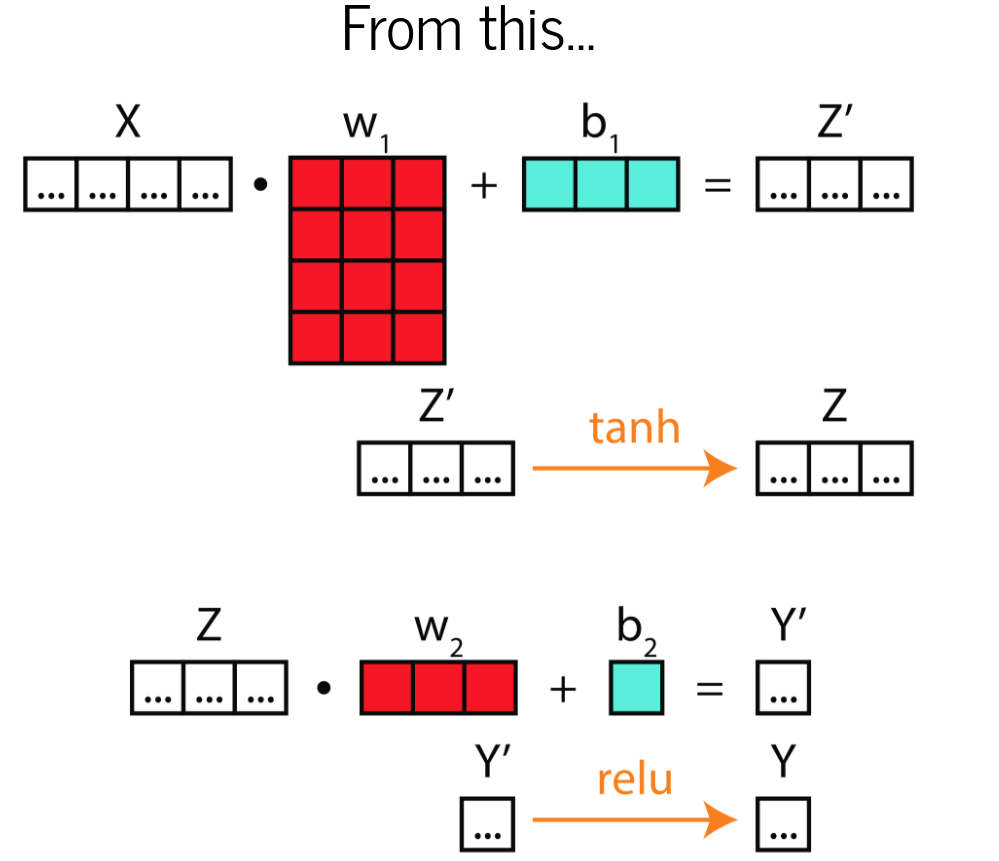
\includegraphics[width = 0.9\textwidth]{im/going_bayesian1.png}
		\caption{Used with kind permission of \mdlink{Eric Ma}{https://ericmjl.github.io/}}
	\end{figure}
\end{frame}

\begin{frame}
	\begin{figure}
		\centering
		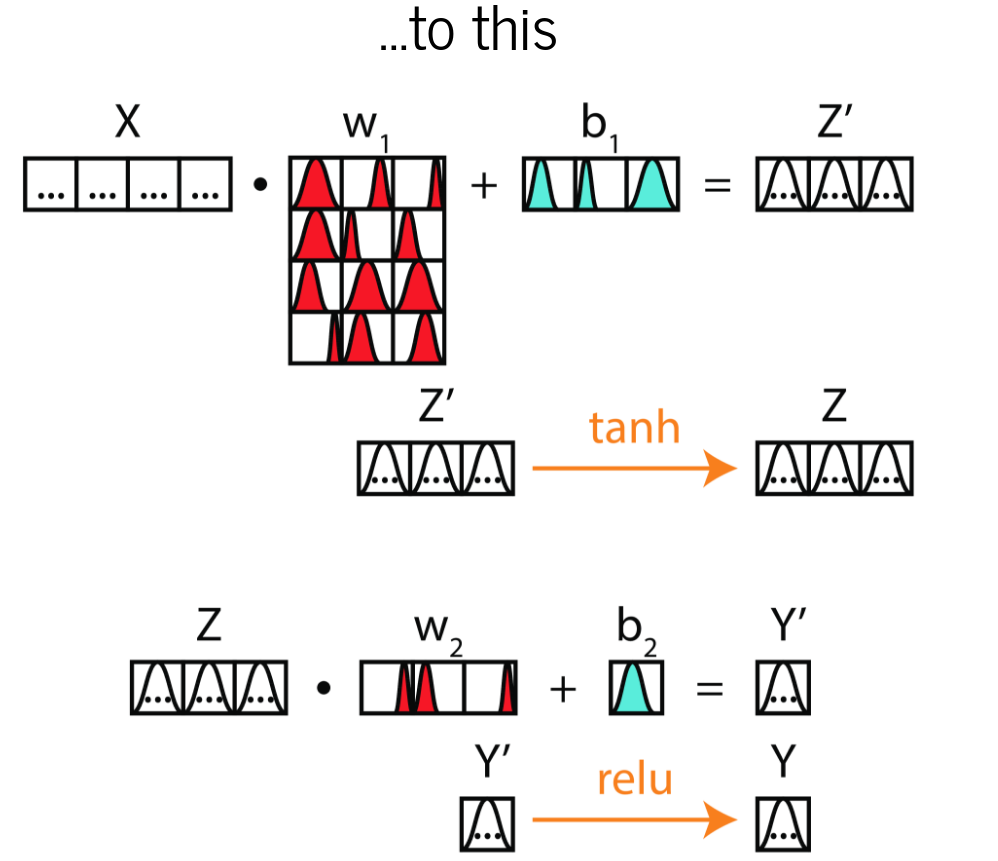
\includegraphics[width = 0.9\textwidth]{im/going_bayesian2.png}
		\caption{Used with kind permission of \mdlink{Eric Ma}{https://ericmjl.github.io/}}
	\end{figure}
\end{frame}

\begin{frame}{Parameters of a Gaussian}
	\begin{figure}
		\fitfigure{im/gaussian_mu_sigma.png}
		\caption{For a Gaussian, we need parameters $\mu$ and $\sigma$}
	\end{figure}
\end{frame}



\subsection{Parameter posterior}

\begin{frame}{Posterior probability}
	The parameter posterior will:
	\begin{itemize}
		\item Enable more samples for prediction $\rightarrow$ uncertainty over prediction
		\item Tell us which parameters have high zero-probability $\rightarrow$ pruning
	\end{itemize}
\end{frame}

\begin{frame}{Loss functions}
	\title{Old and new loss functions}
	\begin{block}{Loss functions}
		\begin{align*}
			  & old \ loss                                                                                                                                                                    \\
			  & = classification \ loss +   \sum_i  \undermath{\lambda  w_i^2}{L2 penalty}                                                                                                    \\
			  &                                                                                                                                                                               \\
			  & new \ loss                                                                                                                                                                    \\		
			  & = classification \ loss +    \sum_i         \undermath{\frac{1}{2}\lambda\mu_i^2 }{L2 penalty}- \undermath{\log\sigma_i + \frac{1}{2}\lambda \sigma_i^2}{penalty on $\sigma$} \\
		\end{align*}
	\end{block}
		
%	\begin{block}{Interpretation}
%		\begin{itemize}
%			\item L2 penalty on the parameter remains
%			\item Loss function on the $\sigma$ 
%		\end{itemize}
%				
%	\end{block}
\end{frame}


\begin{frame}{Intuition}
	\begin{align*}
		  & loss                                                                                                                                                                             \\
		  & = \undermath{classification \ loss + \sum_i \frac{1}{2}\lambda\mu_i^2 }{loss on location of weights} \undermath{-\log\sigma_i + \frac{1}{2}\lambda \sigma_i^2}{loss on $\sigma$} 
	\end{align*}
\end{frame}


\begin{frame}{Summary}
	\begin{itemize}
		\item \textbf{What do we care about?} \\ Uncertainties and pruning
		\item \textbf{How we do that?} \\ Bayesian inference
		\item \textbf{How we do that?} \\ Approximate the parameter posterior
		\item \textbf{How we do that?} \\ Find a $\mu$ and $\sigma$ per parameter
		\item \textbf{How we do that?} \\ Minimize the loss function on the previous slide
	\end{itemize}
\end{frame}


\subsection{Uncertainty}
\begin{frame}{Use entropy as uncertainty metric}
	\begin{figure}
		\fitfigure{/home/rob/Dropbox/ml_projects/weight_uncertainty/weight_uncertainty/im/four_distro_without_entropy.png}
		\caption{Which prediction has least uncertainty?}
	\end{figure}
\end{frame}

\begin{frame}{Use entropy as uncertainty metric}
	\begin{figure}
		\fitfigure{/home/rob/Dropbox/ml_projects/weight_uncertainty/weight_uncertainty/im/four_distro_with_entropy.png}
		\caption{Which prediction has least uncertainty?}
	\end{figure}
\end{frame}

\subsection{Pruning}


\begin{frame}
	\begin{figure}
		\centering
		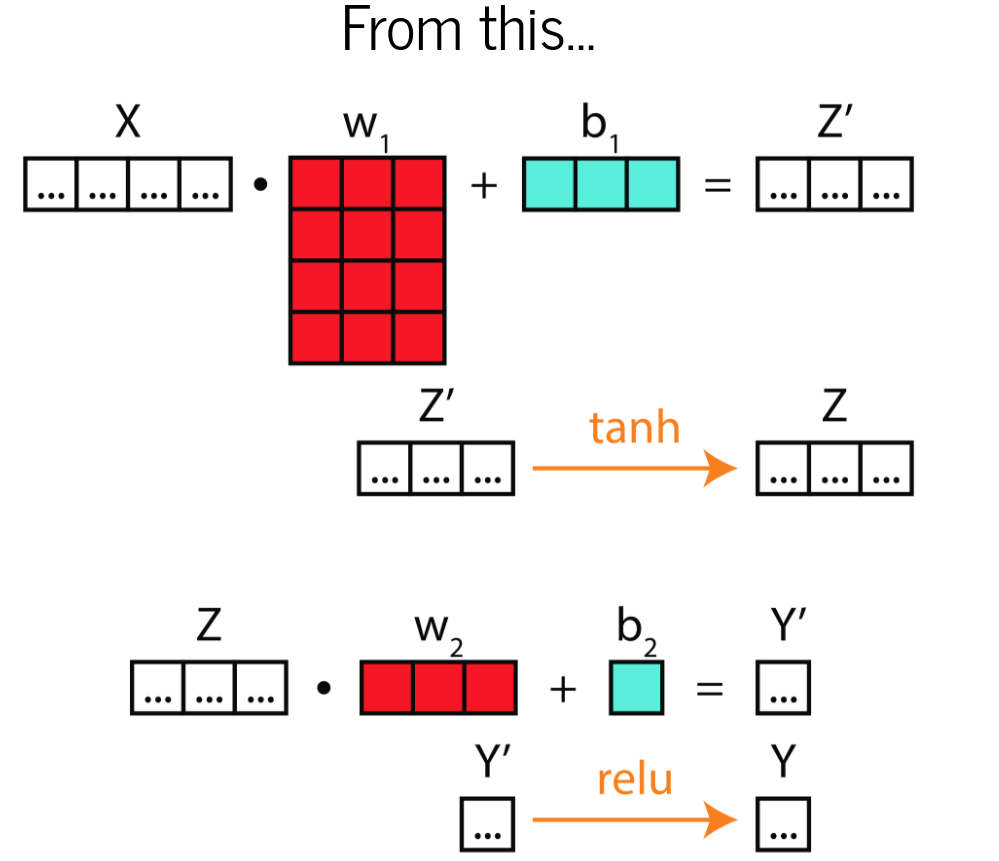
\includegraphics[width = 0.9\textwidth]{im/going_bayesian1.png}
		\caption{Used with kind permission of \mdlink{Eric Ma}{https://ericmjl.github.io/}}
	\end{figure}
\end{frame}

\begin{frame}
	\begin{figure}
		\centering
		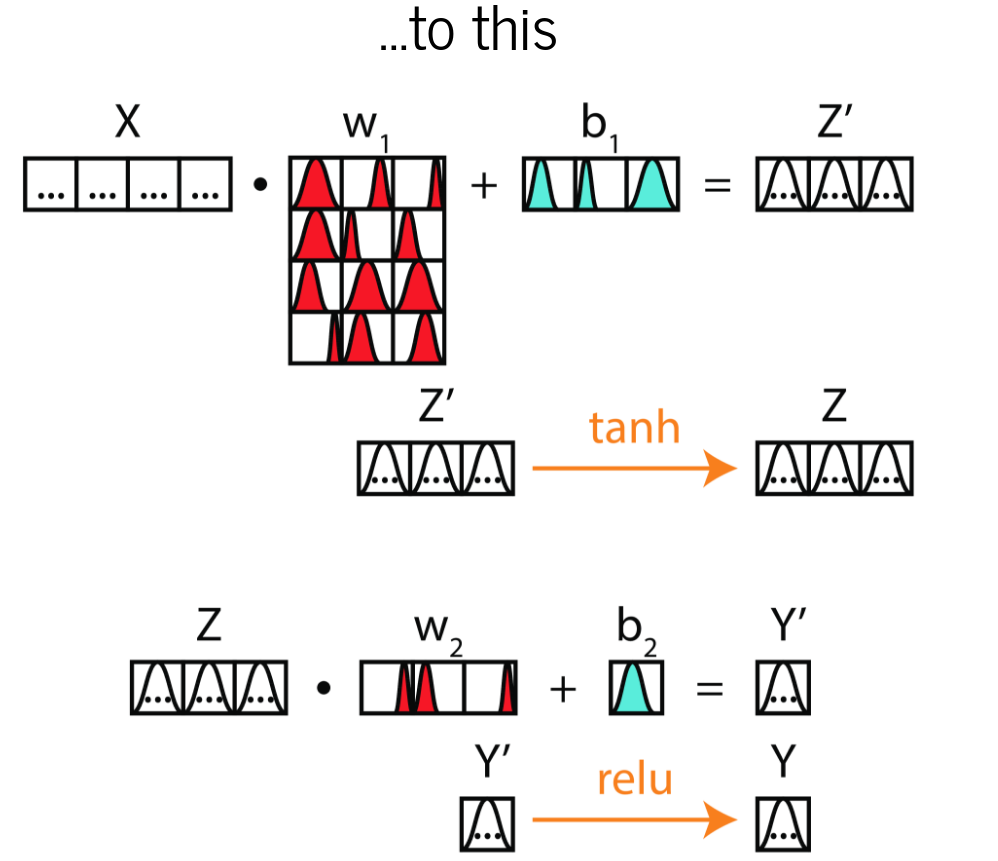
\includegraphics[width = 0.9\textwidth]{im/going_bayesian2.png}
		\caption{Used with kind permission of \mdlink{Eric Ma}{https://ericmjl.github.io/}}
	\end{figure}
\end{frame}

\begin{frame}
	\begin{figure}
		\centering
		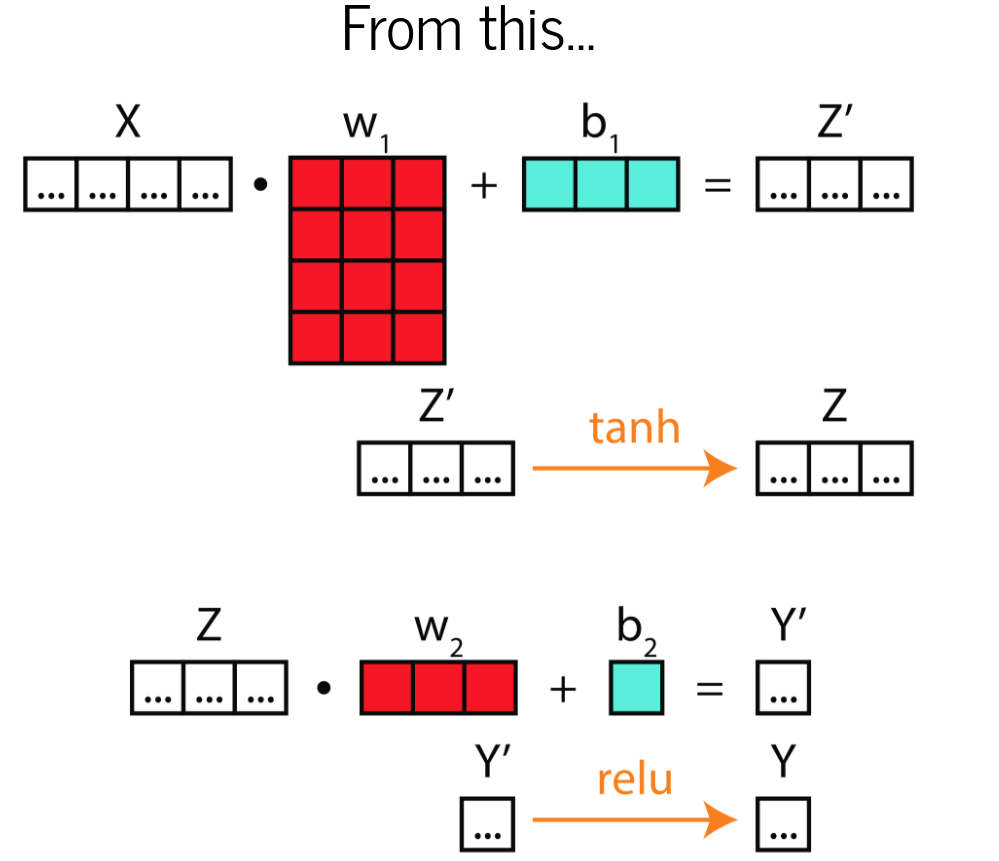
\includegraphics[width = 0.9\textwidth]{im/going_bayesian1.png}
		\caption{Used with kind permission of \mdlink{Eric Ma}{https://ericmjl.github.io/}}
	\end{figure}
\end{frame}

\begin{frame}
	\begin{figure}
		\centering
		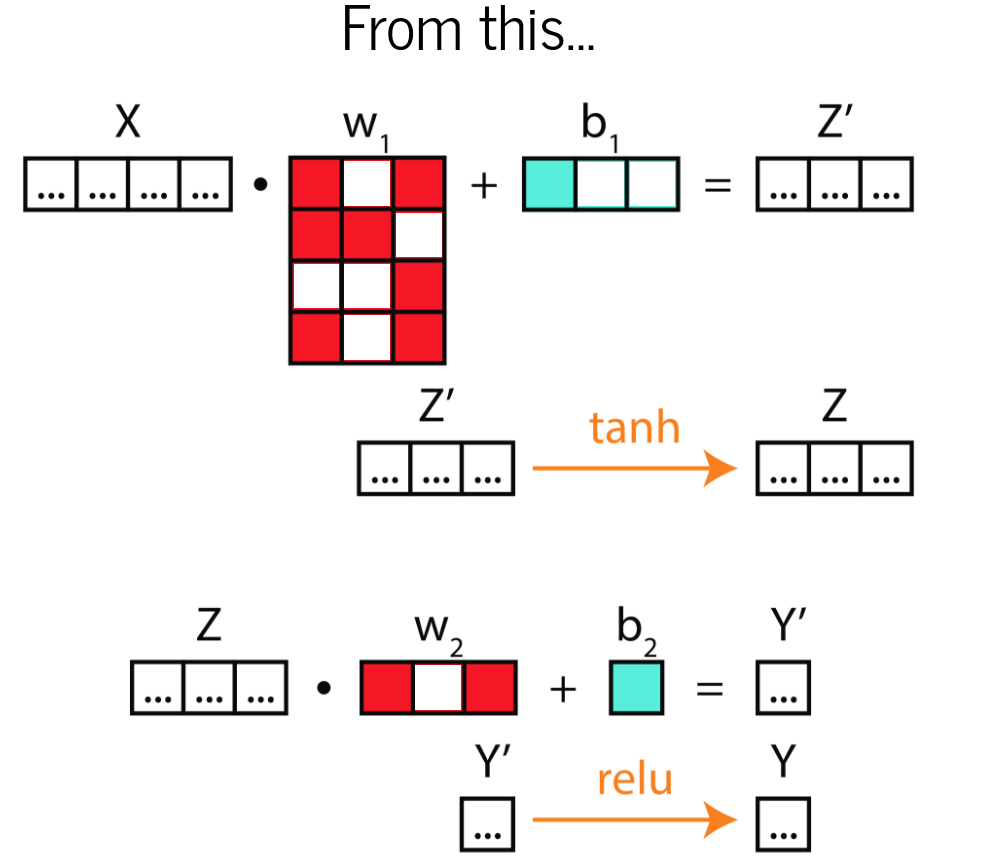
\includegraphics[width = 0.9\textwidth]{im/going_pruning.png}
		\caption{Used with kind permission of \mdlink{Eric Ma}{https://ericmjl.github.io/}}
	\end{figure}
\end{frame}

\begin{frame}{Pruning according to posterior}
	\begin{figure}
		\fitfigure{/home/rob/Dropbox/ml_projects/weight_uncertainty/weight_uncertainty/im/two_distro_pruning.png}
		\caption{Which parameter would you rather prune?}
	\end{figure}
\end{frame}

\section{Experiments and results}
\begin{frame}{Data sets}
	\begin{block}{Fun}
		No deep learning project is complete without \textbf{MNIST}
	\end{block}
			
	\begin{block}{Serious}
		Two most common applications of deep learning:
						
		\begin{itemize}
			\item Image recognition: \textbf{CIFAR10} data set
			\item Time series classification: \textbf{UCR - ECG's}
			      \begin{itemize}
			      	\item Train set only 500 time series $\rightarrow$ Bayesian's don't overfit
			      \end{itemize}
		\end{itemize}
	\end{block}
\end{frame}

\begin{frame}{MNIST examples}
	\begin{figure}
		\fitfigure{im/mnist_examples.png}
		\caption{Examples of MNIST. Train set: 50k samples. Test set: 10k samples}
	\end{figure}
\end{frame}

\begin{frame}{CIFAR examples}
	\begin{figure}
		\fitfigure{im/cifar_examples.png}
		\caption{Examples of CIFAR. Train set: 50k samples. Test set: 10k samples}
	\end{figure}
\end{frame}

\begin{frame}{ECG examples}
	\begin{figure}
		\fitfigure{im/ucr_examples.png}
		\caption{Examples of ECG. Train set: 500 samples. Test set: 4500 samples}
	\end{figure}
\end{frame}


\subsection{Pruning}

\begin{frame}{Remember the model}
	\begin{figure}
		\centering
		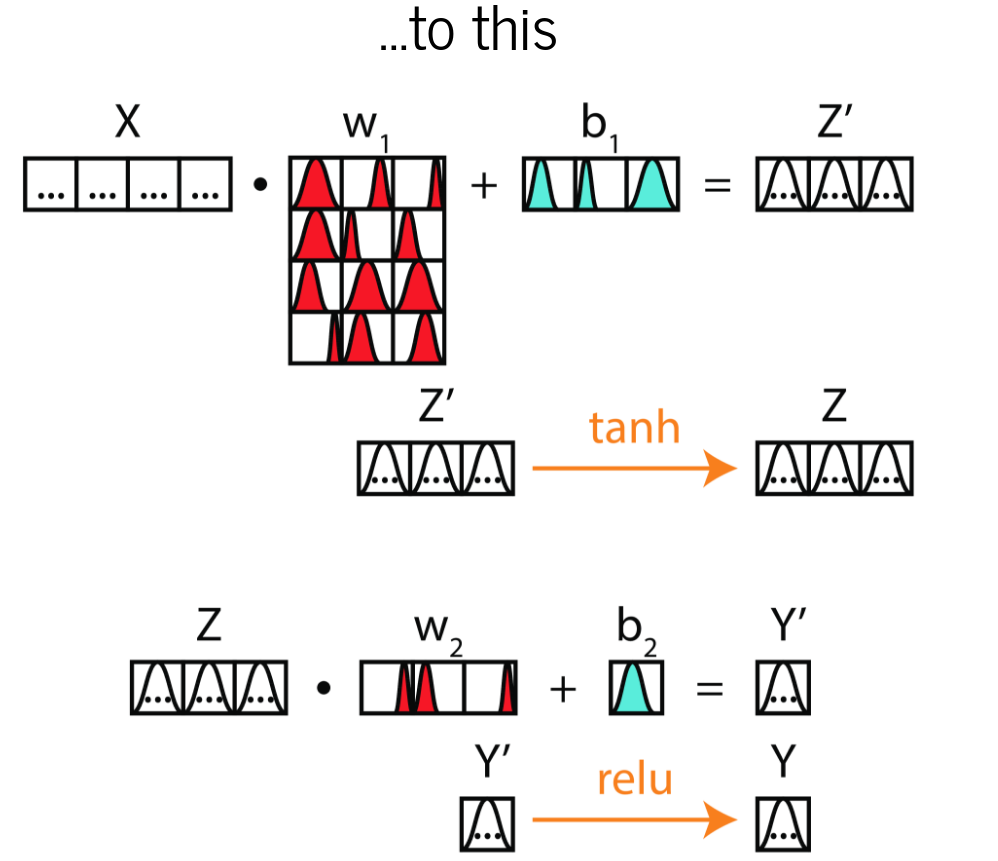
\includegraphics[width = 0.9\textwidth]{im/going_bayesian2.png}
		\caption{Used with kind permission of \mdlink{Eric Ma}{https://ericmjl.github.io/}}
	\end{figure}
\end{frame}

\begin{frame}{Pruning MNIST}
	\begin{figure}
		\fitfigure{/home/rob/Dropbox/ml_projects/weight_uncertainty/weight_uncertainty/im/pruning_curves/mnist_pruning_curve.png}
		\caption{Pruning curve for MNIST}
	\end{figure}
\end{frame}

\begin{frame}{Pruning CIFAR}
	\begin{figure}
		\fitfigure{/home/rob/Dropbox/ml_projects/weight_uncertainty/weight_uncertainty/im/pruning_curves/cifar_pruning_curve.png}
		\caption{Pruning curve for CIFAR}
	\end{figure}
\end{frame}

\begin{frame}{Pruning ECG}
	\begin{figure}
		\fitfigure{/home/rob/Dropbox/ml_projects/weight_uncertainty/weight_uncertainty/im/pruning_curves/ucr_pruning_curve.png}
		\caption{Pruning curve for ECG}
	\end{figure}
\end{frame}

\subsection{Uncertainties}
\begin{frame}{Experiment uncertainty}
	How to mutilate images to raise uncertainty?
	\begin{itemize}
		\item Add noise
		\item Warping
		\item Rotation
	\end{itemize}
\end{frame}

% set to false to speed up compilation
\ifnum1=1
\begin{frame}{Noise}
	\hspace*{-50mm}
	\begin{figure}
		\centering
		\hspace*{-25mm}
		\animategraphics[loop,controls,buttonsize=0.5em,width=1.35\textwidth]{4}{/home/rob/Dropbox/ml_projects/weight_uncertainty/weight_uncertainty/im/mnist/noise/latex/experiment}{0}{49}
		\caption{animation only shows with media plugin (use adobe reader)}
	\end{figure}
\end{frame}

\begin{frame}{Rotation}
	\begin{figure}
		\centering
		\hspace*{-25mm}
		\animategraphics[loop,controls,buttonsize=0.5em,width=1.35\textwidth]{4}{/home/rob/Dropbox/ml_projects/weight_uncertainty/weight_uncertainty/im/mnist/rotation/latex/experiment}{0}{49}
		% TODO ??? fix that this works for 30 samples
		\caption{animation only shows with media plugin (use adobe reader)}
	\end{figure}
\end{frame}

\begin{frame}{Warping}
	\begin{figure}
		\centering
		\hspace*{-25mm}
		\animategraphics[loop,controls,buttonsize=0.5em,width=1.35\textwidth]{4}{/home/rob/Dropbox/ml_projects/weight_uncertainty/weight_uncertainty/im/mnist/warp/latex/experiment}{0}{49}
		% TODO ??? fix that this works for 30 samples
		\caption{animation only shows with media plugin (use adobe reader)}
	\end{figure}
\end{frame}

%\begin{frame}{Warping}
%\begin{figure}
%\centering
%  \animategraphics[loop,controls,width=0.6\linewidth]{2}{/home/rob/Dropbox/ml_projects/weight_uncertainty/weight_uncertainty/im/cifar/noise/latex/experiment}{0}{34}
%  \caption{animation only shows with media plugin (use adobe reader)}
%\end{figure}\end{frame}

\else

\begin{frame}
	Here will be slides with experiments to show uncertainty on CIFAR10 when we add noise or rotate or warp
\end{frame}

\fi

\section{Closing}
\begin{frame}
	\centerline{Take aways}
	\begin{itemize}
		\item Get uncertainty for critical predictions
		\item Robust against adversarial attacks
		\item Prune networks for small memory and small compute
	\end{itemize}
\end{frame}

\begin{frame}
	\centerline{\Huge{Questions?}}
		
	\centerline{  }
	\centerline{\mdlink{robromijnders.github.io}{http://robromijnders.github.io/}}
	\centerline{  }
		
	\begin{block}{Material}
		\mdlink{\url{github.com/RobRomijnders/weight_uncertainty}}{github.com/RobRomijnders/weight_uncertainty}
		\centerline{  }
		\begin{itemize}
			\item All code
			\item Further reading
			\item More explanation
		\end{itemize}
	\end{block}
\end{frame}

\begin{frame}
	\centerline{\Huge{Additional slides}}
\end{frame}

\begin{frame}{Learning the sigma's}
	\begin{figure}
		\fitfigure{/home/rob/Dropbox/ml_projects/weight_uncertainty/weight_uncertainty/im/tensorboard_sample_sigma_pruning.png}
		\caption{The VI objective increases the sigma's by itself!!}
	\end{figure}
		
\end{frame}

\begin{frame}{Loss on $\sigma$}
	What does the loss for $\sigma$ look like?
	\begin{figure}
		\fitfigure{/home/rob/Dropbox/ml_projects/weight_uncertainty/weight_uncertainty/im/loss_sigma.png}
	\end{figure}
\end{frame}

\begin{frame}{Make predictions}
	\begin{block}{Sampling}
		Make multiple predictions with sampled parameters. 
		One can think of this sampling as an ensemble method
	\end{block}   
	\lstinputlisting[language=Python,basicstyle=\small]{code/sampling.py}
\end{frame}


\begin{frame}[shrink=30]{Pseudo code}
	\centerline{Pseudo code for training our neural network}
	\lstinputlisting[language=Python,basicstyle=\small]{code/training.py}
\end{frame}

\begin{frame}[shrink=10]
	\lstinputlisting[language=Python,basicstyle=\small]{code/training_new.py}
\end{frame}

\begin{frame}{Research}
	\begin{block}{Pruning: speed}
		\mdlink{Bayesian compression for deep learning, Louizos @ NIPS2017}{http://papers.nips.cc/paper/6921-bayesian-compression-for-deep-learning.pdf}
	\end{block}
		
	\begin{block}{Uncertainty: adversarial attack}
		\mdlink{Adversarial phenomenon in Bayesian deep learning, Rawat, 2017}{https://arxiv.org/pdf/1711.08244.pdf}
	\end{block}
\end{frame}

\begin{frame}{Gaussian approximation}
	Approximate with a normal distribution
	\begin{itemize}
		\item Captures local structure of the posterior, which indicates the uncertainty
		\item Simple for parameter pruning
	\end{itemize}
	\centerline{  }
	\textbf{\Huge{Anything is better than point estimation !!!}}
\end{frame}

\begin{frame}{Gaussian approximation}
	\begin{figure}
		\fitfigure{im/approximation.png}
		\caption{Any approximation (VI) is better than just a point estimate (MLE)}
	\end{figure}
\end{frame}

\begin{frame}{Bernoulli approximations}
	\begin{figure}
		\fitfigure{im/gaussian_or_bernoulli.png}
		\caption{Bernoulli approximation does not capture local properties}
	\end{figure}
\end{frame}

\begin{frame}{Adding noise}
	\begin{figure}
		\centering
		\hspace*{-25mm}
		\animategraphics[loop,controls,buttonsize=0.5em,width=1.35\textwidth]{4}{/home/rob/Dropbox/ml_projects/weight_uncertainty/weight_uncertainty/im/cifar/noise/latex/experiment}{0}{34}
		\caption{animation only shows with media plugin (use adobe reader)}
	\end{figure}
\end{frame}

\end{document}